\documentclass[twoside]{book}

% Packages required by doxygen
\usepackage{fixltx2e}
\usepackage{calc}
\usepackage{doxygen}
\usepackage[export]{adjustbox} % also loads graphicx
\usepackage{graphicx}
\usepackage[utf8]{inputenc}
\usepackage{makeidx}
\usepackage{multicol}
\usepackage{multirow}
\PassOptionsToPackage{warn}{textcomp}
\usepackage{textcomp}
\usepackage[nointegrals]{wasysym}
\usepackage[table]{xcolor}

% NLS support packages
\usepackage[T2A]{fontenc}
\usepackage[russian]{babel}

% Font selection
\usepackage[T1]{fontenc}
\usepackage[scaled=.90]{helvet}
\usepackage{courier}
\usepackage{amssymb}
\usepackage{sectsty}
\renewcommand{\familydefault}{\sfdefault}
\allsectionsfont{%
  \fontseries{bc}\selectfont%
  \color{darkgray}%
}
\renewcommand{\DoxyLabelFont}{%
  \fontseries{bc}\selectfont%
  \color{darkgray}%
}
\newcommand{\+}{\discretionary{\mbox{\scriptsize$\hookleftarrow$}}{}{}}

% Page & text layout
\usepackage{geometry}
\geometry{%
  a4paper,%
  top=2.5cm,%
  bottom=2.5cm,%
  left=2.5cm,%
  right=2.5cm%
}
\tolerance=750
\hfuzz=15pt
\hbadness=750
\setlength{\emergencystretch}{15pt}
\setlength{\parindent}{0cm}
\setlength{\parskip}{3ex plus 2ex minus 2ex}
\makeatletter
\renewcommand{\paragraph}{%
  \@startsection{paragraph}{4}{0ex}{-1.0ex}{1.0ex}{%
    \normalfont\normalsize\bfseries\SS@parafont%
  }%
}
\renewcommand{\subparagraph}{%
  \@startsection{subparagraph}{5}{0ex}{-1.0ex}{1.0ex}{%
    \normalfont\normalsize\bfseries\SS@subparafont%
  }%
}
\makeatother

% Headers & footers
\usepackage{fancyhdr}
\pagestyle{fancyplain}
\fancyhead[LE]{\fancyplain{}{\bfseries\thepage}}
\fancyhead[CE]{\fancyplain{}{}}
\fancyhead[RE]{\fancyplain{}{\bfseries\leftmark}}
\fancyhead[LO]{\fancyplain{}{\bfseries\rightmark}}
\fancyhead[CO]{\fancyplain{}{}}
\fancyhead[RO]{\fancyplain{}{\bfseries\thepage}}
\fancyfoot[LE]{\fancyplain{}{}}
\fancyfoot[CE]{\fancyplain{}{}}
\fancyfoot[RE]{\fancyplain{}{\bfseries\scriptsize Создано системой Doxygen }}
\fancyfoot[LO]{\fancyplain{}{\bfseries\scriptsize Создано системой Doxygen }}
\fancyfoot[CO]{\fancyplain{}{}}
\fancyfoot[RO]{\fancyplain{}{}}
\renewcommand{\footrulewidth}{0.4pt}
\renewcommand{\chaptermark}[1]{%
  \markboth{#1}{}%
}
\renewcommand{\sectionmark}[1]{%
  \markright{\thesection\ #1}%
}

% Indices & bibliography
\usepackage{natbib}
\usepackage[titles]{tocloft}
\setcounter{tocdepth}{3}
\setcounter{secnumdepth}{5}
\makeindex

% Hyperlinks (required, but should be loaded last)
\usepackage{ifpdf}
\ifpdf
  \usepackage[pdftex,pagebackref=true]{hyperref}
\else
  \usepackage[ps2pdf,pagebackref=true]{hyperref}
\fi
\hypersetup{%
  colorlinks=true,%
  linkcolor=blue,%
  citecolor=blue,%
  unicode%
}

% Custom commands
\newcommand{\clearemptydoublepage}{%
  \newpage{\pagestyle{empty}\cleardoublepage}%
}

\usepackage{caption}
\captionsetup{labelsep=space,justification=centering,font={bf},singlelinecheck=off,skip=4pt,position=top}

%===== C O N T E N T S =====

\begin{document}

% Titlepage & ToC
\hypersetup{pageanchor=false,
             bookmarksnumbered=true,
             pdfencoding=unicode
            }
\pagenumbering{roman}
\begin{titlepage}
\vspace*{7cm}
\begin{center}%
{\Large Домашнее задание №3.1 }\\
\vspace*{1cm}
{\large Создано системой Doxygen 1.8.11}\\
\end{center}
\end{titlepage}
\clearemptydoublepage
\tableofcontents
\clearemptydoublepage
\pagenumbering{arabic}
\hypersetup{pageanchor=true}

%--- Begin generated contents ---
\chapter{Иерархический список классов}
\section{Иерархия классов}
Иерархия классов.\begin{DoxyCompactList}
\item \contentsline{section}{Word}{\pageref{classWord}}{}
\begin{DoxyCompactList}
\item \contentsline{section}{Sentence}{\pageref{classSentence}}{}
\end{DoxyCompactList}
\end{DoxyCompactList}

\chapter{Алфавитный указатель классов}
\section{Классы}
Классы с их кратким описанием.\begin{DoxyCompactList}
\item\contentsline{section}{\hyperlink{classSentence}{Sentence} }{\pageref{classSentence}}{}
\item\contentsline{section}{\hyperlink{classWord}{Word} }{\pageref{classWord}}{}
\end{DoxyCompactList}

\chapter{Список файлов}
\section{Файлы}
Полный список файлов.\begin{DoxyCompactList}
\item\contentsline{section}{\hyperlink{HW3_81_8cpp}{H\+W3.\+1.\+cpp} }{\pageref{HW3_81_8cpp}}{}
\item\contentsline{section}{\hyperlink{HW3_81_8h}{H\+W3.\+1.\+h} }{\pageref{HW3_81_8h}}{}
\item\contentsline{section}{\hyperlink{HW3_81_8hpp}{H\+W3.\+1.\+hpp} }{\pageref{HW3_81_8hpp}}{}
\end{DoxyCompactList}

\chapter{Классы}
\hypertarget{classSentence}{}\section{Класс Sentence}
\label{classSentence}\index{Sentence@{Sentence}}


{\ttfamily \#include $<$H\+W3.\+1.\+h$>$}



Граф наследования\+:Sentence\+:\nopagebreak
\begin{figure}[H]
\begin{center}
\leavevmode
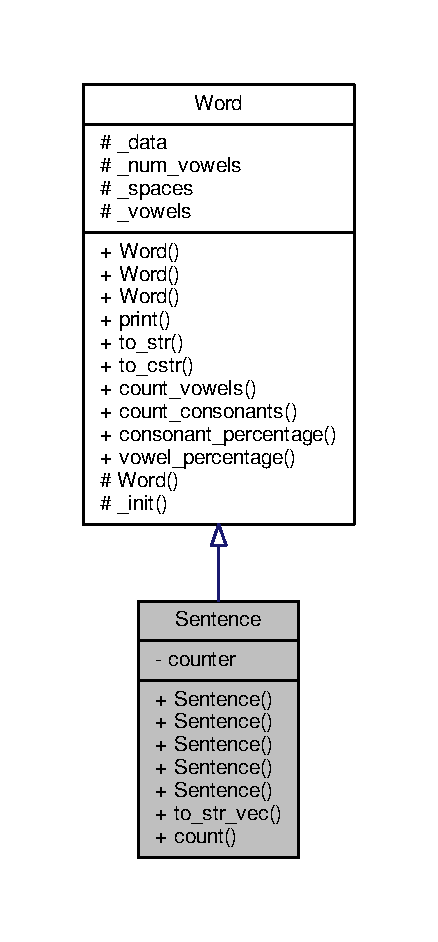
\includegraphics[width=210pt]{classSentence__inherit__graph}
\end{center}
\end{figure}


Граф связей класса Sentence\+:\nopagebreak
\begin{figure}[H]
\begin{center}
\leavevmode
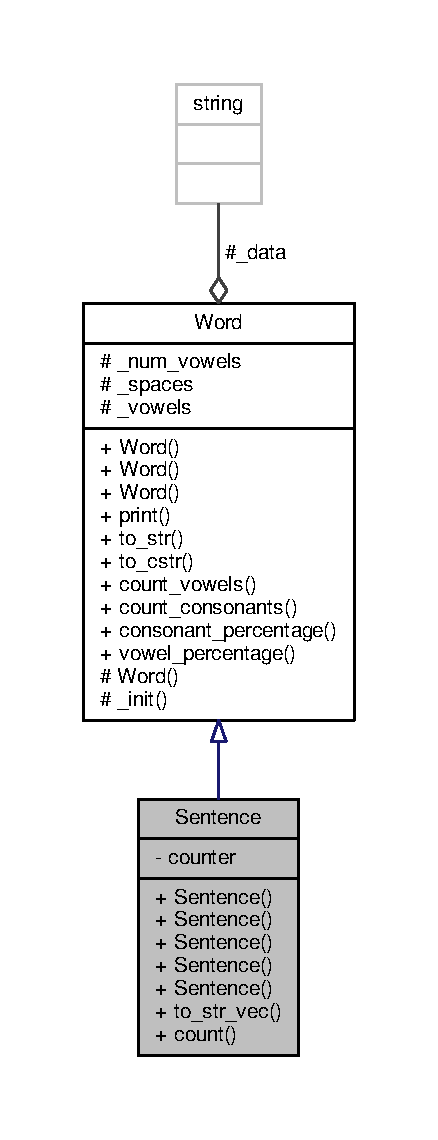
\includegraphics[width=210pt]{classSentence__coll__graph}
\end{center}
\end{figure}
\subsection*{Открытые члены}
\begin{DoxyCompactItemize}
\item 
\hyperlink{classSentence_a3048354db110b3c53f22a0e73f8a2873}{Sentence} (const \hyperlink{classSentence}{Sentence} \&sen)
\item 
\hyperlink{classSentence_abd9587431f7092cacbafbab3deb54eac}{Sentence} (string s)
\item 
\hyperlink{classSentence_af800b4dfcfb0e36de291ce3bd1c4b151}{Sentence} (const char $\ast$s)
\item 
\hyperlink{classSentence_abfcb3ae5846f46f71866330e54288f6e}{Sentence} (\hyperlink{classWord}{Word} w)
\item 
\hyperlink{classSentence_a6735a441c8edf1eab29687f70ce6697e}{Sentence} (vector$<$ string $>$ v)
\item 
vector$<$ string $>$ \hyperlink{classSentence_a1c2e3f16dbbaf2446a1d1f5ddac694d3}{to\+\_\+str\+\_\+vec} ()
\item 
size\+\_\+t \hyperlink{classSentence_a9775e8e13161099b03b281a31fcdf050}{count} ()
\end{DoxyCompactItemize}
\subsection*{Закрытые данные}
\begin{DoxyCompactItemize}
\item 
size\+\_\+t \hyperlink{classSentence_a5ad2286635c8e8620085b48f81ae2457}{counter}
\end{DoxyCompactItemize}
\subsection*{Дополнительные унаследованные члены}


\subsection{Конструктор(ы)}
\index{Sentence@{Sentence}!Sentence@{Sentence}}
\index{Sentence@{Sentence}!Sentence@{Sentence}}
\subsubsection[{\texorpdfstring{Sentence(const Sentence \&sen)}{Sentence(const Sentence &sen)}}]{\setlength{\rightskip}{0pt plus 5cm}Sentence\+::\+Sentence (
\begin{DoxyParamCaption}
\item[{const {\bf Sentence} \&}]{sen}
\end{DoxyParamCaption}
)\hspace{0.3cm}{\ttfamily [inline]}}\hypertarget{classSentence_a3048354db110b3c53f22a0e73f8a2873}{}\label{classSentence_a3048354db110b3c53f22a0e73f8a2873}
\index{Sentence@{Sentence}!Sentence@{Sentence}}
\index{Sentence@{Sentence}!Sentence@{Sentence}}
\subsubsection[{\texorpdfstring{Sentence(string s)}{Sentence(string s)}}]{\setlength{\rightskip}{0pt plus 5cm}Sentence\+::\+Sentence (
\begin{DoxyParamCaption}
\item[{string}]{s}
\end{DoxyParamCaption}
)}\hypertarget{classSentence_abd9587431f7092cacbafbab3deb54eac}{}\label{classSentence_abd9587431f7092cacbafbab3deb54eac}
\index{Sentence@{Sentence}!Sentence@{Sentence}}
\index{Sentence@{Sentence}!Sentence@{Sentence}}
\subsubsection[{\texorpdfstring{Sentence(const char $\ast$s)}{Sentence(const char *s)}}]{\setlength{\rightskip}{0pt plus 5cm}Sentence\+::\+Sentence (
\begin{DoxyParamCaption}
\item[{const char $\ast$}]{s}
\end{DoxyParamCaption}
)}\hypertarget{classSentence_af800b4dfcfb0e36de291ce3bd1c4b151}{}\label{classSentence_af800b4dfcfb0e36de291ce3bd1c4b151}
\index{Sentence@{Sentence}!Sentence@{Sentence}}
\index{Sentence@{Sentence}!Sentence@{Sentence}}
\subsubsection[{\texorpdfstring{Sentence(\+Word w)}{Sentence(Word w)}}]{\setlength{\rightskip}{0pt plus 5cm}Sentence\+::\+Sentence (
\begin{DoxyParamCaption}
\item[{{\bf Word}}]{w}
\end{DoxyParamCaption}
)}\hypertarget{classSentence_abfcb3ae5846f46f71866330e54288f6e}{}\label{classSentence_abfcb3ae5846f46f71866330e54288f6e}
\index{Sentence@{Sentence}!Sentence@{Sentence}}
\index{Sentence@{Sentence}!Sentence@{Sentence}}
\subsubsection[{\texorpdfstring{Sentence(vector$<$ string $>$ v)}{Sentence(vector< string > v)}}]{\setlength{\rightskip}{0pt plus 5cm}Sentence\+::\+Sentence (
\begin{DoxyParamCaption}
\item[{vector$<$ string $>$}]{v}
\end{DoxyParamCaption}
)}\hypertarget{classSentence_a6735a441c8edf1eab29687f70ce6697e}{}\label{classSentence_a6735a441c8edf1eab29687f70ce6697e}


\subsection{Методы}
\index{Sentence@{Sentence}!count@{count}}
\index{count@{count}!Sentence@{Sentence}}
\subsubsection[{\texorpdfstring{count()}{count()}}]{\setlength{\rightskip}{0pt plus 5cm}size\+\_\+t Sentence\+::count (
\begin{DoxyParamCaption}
{}
\end{DoxyParamCaption}
)}\hypertarget{classSentence_a9775e8e13161099b03b281a31fcdf050}{}\label{classSentence_a9775e8e13161099b03b281a31fcdf050}
\index{Sentence@{Sentence}!to\+\_\+str\+\_\+vec@{to\+\_\+str\+\_\+vec}}
\index{to\+\_\+str\+\_\+vec@{to\+\_\+str\+\_\+vec}!Sentence@{Sentence}}
\subsubsection[{\texorpdfstring{to\+\_\+str\+\_\+vec()}{to_str_vec()}}]{\setlength{\rightskip}{0pt plus 5cm}vector$<$ string $>$ Sentence\+::to\+\_\+str\+\_\+vec (
\begin{DoxyParamCaption}
{}
\end{DoxyParamCaption}
)}\hypertarget{classSentence_a1c2e3f16dbbaf2446a1d1f5ddac694d3}{}\label{classSentence_a1c2e3f16dbbaf2446a1d1f5ddac694d3}


\subsection{Данные класса}
\index{Sentence@{Sentence}!counter@{counter}}
\index{counter@{counter}!Sentence@{Sentence}}
\subsubsection[{\texorpdfstring{counter}{counter}}]{\setlength{\rightskip}{0pt plus 5cm}size\+\_\+t Sentence\+::counter\hspace{0.3cm}{\ttfamily [private]}}\hypertarget{classSentence_a5ad2286635c8e8620085b48f81ae2457}{}\label{classSentence_a5ad2286635c8e8620085b48f81ae2457}


Объявления и описания членов классов находятся в файлах\+:\begin{DoxyCompactItemize}
\item 
\hyperlink{HW3_81_8h}{H\+W3.\+1.\+h}\item 
\hyperlink{HW3_81_8hpp}{H\+W3.\+1.\+hpp}\end{DoxyCompactItemize}

\hypertarget{classWord}{}\section{Класс Word}
\label{classWord}\index{Word@{Word}}


{\ttfamily \#include $<$H\+W3.\+1.\+h$>$}



Граф наследования\+:Word\+:\nopagebreak
\begin{figure}[H]
\begin{center}
\leavevmode
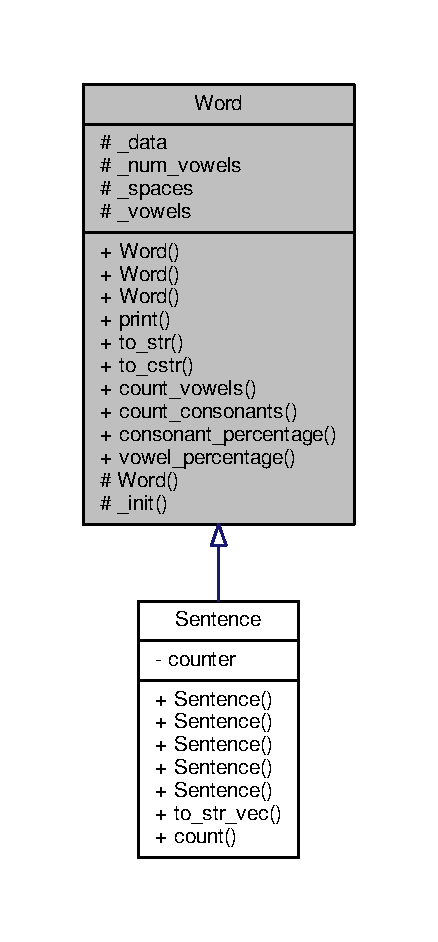
\includegraphics[width=210pt]{classWord__inherit__graph}
\end{center}
\end{figure}


Граф связей класса Word\+:\nopagebreak
\begin{figure}[H]
\begin{center}
\leavevmode
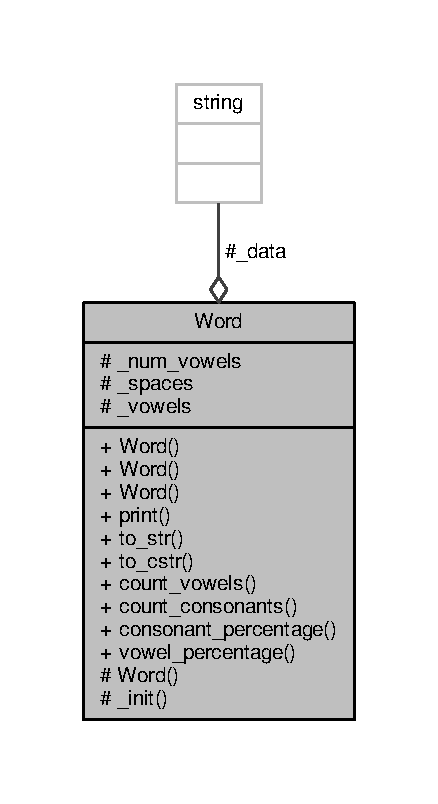
\includegraphics[width=210pt]{classWord__coll__graph}
\end{center}
\end{figure}
\subsection*{Открытые члены}
\begin{DoxyCompactItemize}
\item 
\hyperlink{classWord_ac6f487c9336bcddcdca8d149d7c3ccb5}{Word} (const \hyperlink{classWord}{Word} \&w)
\item 
\hyperlink{classWord_a86290013f4b538ae7aeef2720fc240ee}{Word} (string s)
\item 
\hyperlink{classWord_a7f27bc6191af83d7fce1a16838081872}{Word} (const char $\ast$s)
\item 
void \hyperlink{classWord_a71f14ead088ecaf6941f9c91b75c25c9}{print} ()
\item 
string \hyperlink{classWord_a75606ad31d249369f93c7ad83a6798e4}{to\+\_\+str} ()
\item 
void \hyperlink{classWord_ab02157e87243aad185d0f8f4c33862a4}{to\+\_\+cstr} (char $\ast$arr)
\item 
size\+\_\+t \hyperlink{classWord_a450a0259aba9504e3f7d6d4fa363cd7a}{count\+\_\+vowels} ()
\item 
size\+\_\+t \hyperlink{classWord_a61af6d4fa64014ce6d237657d058c57f}{count\+\_\+consonants} ()
\item 
float \hyperlink{classWord_aa19ec4d5e0b9ab9cd5f3cf54d9c4c106}{consonant\+\_\+percentage} ()
\item 
float \hyperlink{classWord_aa8e6259183ceaa15497d704c4c92b70a}{vowel\+\_\+percentage} ()
\end{DoxyCompactItemize}
\subsection*{Защищенные члены}
\begin{DoxyCompactItemize}
\item 
\hyperlink{classWord_a17baf7109d46beb48d5b469f3baedc48}{Word} ()
\item 
void \hyperlink{classWord_a6a557d92243a1a4aa0f7a874b3c66a22}{\+\_\+init} (const char $\ast$s)
\end{DoxyCompactItemize}
\subsection*{Защищенные данные}
\begin{DoxyCompactItemize}
\item 
string \hyperlink{classWord_adc46545d81f0158074f941731ae5bb52}{\+\_\+data}
\item 
size\+\_\+t \hyperlink{classWord_a95a4914370c936b524ab21ff42177fb8}{\+\_\+num\+\_\+vowels}
\item 
size\+\_\+t \hyperlink{classWord_afffea82d937c3486011b409bcff4c938}{\+\_\+spaces}
\end{DoxyCompactItemize}
\subsection*{Статические защищенные данные}
\begin{DoxyCompactItemize}
\item 
static constexpr char \hyperlink{classWord_a5c77b083065c497224d3ad4b0b5958de}{\+\_\+vowels} \mbox{[}$\,$\mbox{]} = \char`\"{}A\+E\+U\+I\+Oaeuio\char`\"{}
\end{DoxyCompactItemize}


\subsection{Конструктор(ы)}
\index{Word@{Word}!Word@{Word}}
\index{Word@{Word}!Word@{Word}}
\subsubsection[{\texorpdfstring{Word()}{Word()}}]{\setlength{\rightskip}{0pt plus 5cm}Word\+::\+Word (
\begin{DoxyParamCaption}
{}
\end{DoxyParamCaption}
)\hspace{0.3cm}{\ttfamily [inline]}, {\ttfamily [protected]}}\hypertarget{classWord_a17baf7109d46beb48d5b469f3baedc48}{}\label{classWord_a17baf7109d46beb48d5b469f3baedc48}
\index{Word@{Word}!Word@{Word}}
\index{Word@{Word}!Word@{Word}}
\subsubsection[{\texorpdfstring{Word(const Word \&w)}{Word(const Word &w)}}]{\setlength{\rightskip}{0pt plus 5cm}Word\+::\+Word (
\begin{DoxyParamCaption}
\item[{const {\bf Word} \&}]{w}
\end{DoxyParamCaption}
)\hspace{0.3cm}{\ttfamily [inline]}}\hypertarget{classWord_ac6f487c9336bcddcdca8d149d7c3ccb5}{}\label{classWord_ac6f487c9336bcddcdca8d149d7c3ccb5}
\index{Word@{Word}!Word@{Word}}
\index{Word@{Word}!Word@{Word}}
\subsubsection[{\texorpdfstring{Word(string s)}{Word(string s)}}]{\setlength{\rightskip}{0pt plus 5cm}Word\+::\+Word (
\begin{DoxyParamCaption}
\item[{string}]{s}
\end{DoxyParamCaption}
)}\hypertarget{classWord_a86290013f4b538ae7aeef2720fc240ee}{}\label{classWord_a86290013f4b538ae7aeef2720fc240ee}
\index{Word@{Word}!Word@{Word}}
\index{Word@{Word}!Word@{Word}}
\subsubsection[{\texorpdfstring{Word(const char $\ast$s)}{Word(const char *s)}}]{\setlength{\rightskip}{0pt plus 5cm}Word\+::\+Word (
\begin{DoxyParamCaption}
\item[{const char $\ast$}]{s}
\end{DoxyParamCaption}
)}\hypertarget{classWord_a7f27bc6191af83d7fce1a16838081872}{}\label{classWord_a7f27bc6191af83d7fce1a16838081872}


\subsection{Методы}
\index{Word@{Word}!\+\_\+init@{\+\_\+init}}
\index{\+\_\+init@{\+\_\+init}!Word@{Word}}
\subsubsection[{\texorpdfstring{\+\_\+init(const char $\ast$s)}{_init(const char *s)}}]{\setlength{\rightskip}{0pt plus 5cm}void Word\+::\+\_\+init (
\begin{DoxyParamCaption}
\item[{const char $\ast$}]{s}
\end{DoxyParamCaption}
)\hspace{0.3cm}{\ttfamily [protected]}}\hypertarget{classWord_a6a557d92243a1a4aa0f7a874b3c66a22}{}\label{classWord_a6a557d92243a1a4aa0f7a874b3c66a22}
\index{Word@{Word}!consonant\+\_\+percentage@{consonant\+\_\+percentage}}
\index{consonant\+\_\+percentage@{consonant\+\_\+percentage}!Word@{Word}}
\subsubsection[{\texorpdfstring{consonant\+\_\+percentage()}{consonant_percentage()}}]{\setlength{\rightskip}{0pt plus 5cm}float Word\+::consonant\+\_\+percentage (
\begin{DoxyParamCaption}
{}
\end{DoxyParamCaption}
)}\hypertarget{classWord_aa19ec4d5e0b9ab9cd5f3cf54d9c4c106}{}\label{classWord_aa19ec4d5e0b9ab9cd5f3cf54d9c4c106}
\index{Word@{Word}!count\+\_\+consonants@{count\+\_\+consonants}}
\index{count\+\_\+consonants@{count\+\_\+consonants}!Word@{Word}}
\subsubsection[{\texorpdfstring{count\+\_\+consonants()}{count_consonants()}}]{\setlength{\rightskip}{0pt plus 5cm}size\+\_\+t Word\+::count\+\_\+consonants (
\begin{DoxyParamCaption}
{}
\end{DoxyParamCaption}
)}\hypertarget{classWord_a61af6d4fa64014ce6d237657d058c57f}{}\label{classWord_a61af6d4fa64014ce6d237657d058c57f}
\index{Word@{Word}!count\+\_\+vowels@{count\+\_\+vowels}}
\index{count\+\_\+vowels@{count\+\_\+vowels}!Word@{Word}}
\subsubsection[{\texorpdfstring{count\+\_\+vowels()}{count_vowels()}}]{\setlength{\rightskip}{0pt plus 5cm}size\+\_\+t Word\+::count\+\_\+vowels (
\begin{DoxyParamCaption}
{}
\end{DoxyParamCaption}
)}\hypertarget{classWord_a450a0259aba9504e3f7d6d4fa363cd7a}{}\label{classWord_a450a0259aba9504e3f7d6d4fa363cd7a}
\index{Word@{Word}!print@{print}}
\index{print@{print}!Word@{Word}}
\subsubsection[{\texorpdfstring{print()}{print()}}]{\setlength{\rightskip}{0pt plus 5cm}void Word\+::print (
\begin{DoxyParamCaption}
{}
\end{DoxyParamCaption}
)}\hypertarget{classWord_a71f14ead088ecaf6941f9c91b75c25c9}{}\label{classWord_a71f14ead088ecaf6941f9c91b75c25c9}
\index{Word@{Word}!to\+\_\+cstr@{to\+\_\+cstr}}
\index{to\+\_\+cstr@{to\+\_\+cstr}!Word@{Word}}
\subsubsection[{\texorpdfstring{to\+\_\+cstr(char $\ast$arr)}{to_cstr(char *arr)}}]{\setlength{\rightskip}{0pt plus 5cm}void Word\+::to\+\_\+cstr (
\begin{DoxyParamCaption}
\item[{char $\ast$}]{arr}
\end{DoxyParamCaption}
)}\hypertarget{classWord_ab02157e87243aad185d0f8f4c33862a4}{}\label{classWord_ab02157e87243aad185d0f8f4c33862a4}
\index{Word@{Word}!to\+\_\+str@{to\+\_\+str}}
\index{to\+\_\+str@{to\+\_\+str}!Word@{Word}}
\subsubsection[{\texorpdfstring{to\+\_\+str()}{to_str()}}]{\setlength{\rightskip}{0pt plus 5cm}string Word\+::to\+\_\+str (
\begin{DoxyParamCaption}
{}
\end{DoxyParamCaption}
)}\hypertarget{classWord_a75606ad31d249369f93c7ad83a6798e4}{}\label{classWord_a75606ad31d249369f93c7ad83a6798e4}
\index{Word@{Word}!vowel\+\_\+percentage@{vowel\+\_\+percentage}}
\index{vowel\+\_\+percentage@{vowel\+\_\+percentage}!Word@{Word}}
\subsubsection[{\texorpdfstring{vowel\+\_\+percentage()}{vowel_percentage()}}]{\setlength{\rightskip}{0pt plus 5cm}float Word\+::vowel\+\_\+percentage (
\begin{DoxyParamCaption}
{}
\end{DoxyParamCaption}
)}\hypertarget{classWord_aa8e6259183ceaa15497d704c4c92b70a}{}\label{classWord_aa8e6259183ceaa15497d704c4c92b70a}


\subsection{Данные класса}
\index{Word@{Word}!\+\_\+data@{\+\_\+data}}
\index{\+\_\+data@{\+\_\+data}!Word@{Word}}
\subsubsection[{\texorpdfstring{\+\_\+data}{_data}}]{\setlength{\rightskip}{0pt plus 5cm}string Word\+::\+\_\+data\hspace{0.3cm}{\ttfamily [protected]}}\hypertarget{classWord_adc46545d81f0158074f941731ae5bb52}{}\label{classWord_adc46545d81f0158074f941731ae5bb52}
\index{Word@{Word}!\+\_\+num\+\_\+vowels@{\+\_\+num\+\_\+vowels}}
\index{\+\_\+num\+\_\+vowels@{\+\_\+num\+\_\+vowels}!Word@{Word}}
\subsubsection[{\texorpdfstring{\+\_\+num\+\_\+vowels}{_num_vowels}}]{\setlength{\rightskip}{0pt plus 5cm}size\+\_\+t Word\+::\+\_\+num\+\_\+vowels\hspace{0.3cm}{\ttfamily [protected]}}\hypertarget{classWord_a95a4914370c936b524ab21ff42177fb8}{}\label{classWord_a95a4914370c936b524ab21ff42177fb8}
\index{Word@{Word}!\+\_\+spaces@{\+\_\+spaces}}
\index{\+\_\+spaces@{\+\_\+spaces}!Word@{Word}}
\subsubsection[{\texorpdfstring{\+\_\+spaces}{_spaces}}]{\setlength{\rightskip}{0pt plus 5cm}size\+\_\+t Word\+::\+\_\+spaces\hspace{0.3cm}{\ttfamily [protected]}}\hypertarget{classWord_afffea82d937c3486011b409bcff4c938}{}\label{classWord_afffea82d937c3486011b409bcff4c938}
\index{Word@{Word}!\+\_\+vowels@{\+\_\+vowels}}
\index{\+\_\+vowels@{\+\_\+vowels}!Word@{Word}}
\subsubsection[{\texorpdfstring{\+\_\+vowels}{_vowels}}]{\setlength{\rightskip}{0pt plus 5cm}constexpr char Word\+::\+\_\+vowels = \char`\"{}A\+E\+U\+I\+Oaeuio\char`\"{}\hspace{0.3cm}{\ttfamily [static]}, {\ttfamily [protected]}}\hypertarget{classWord_a5c77b083065c497224d3ad4b0b5958de}{}\label{classWord_a5c77b083065c497224d3ad4b0b5958de}


Объявления и описания членов классов находятся в файлах\+:\begin{DoxyCompactItemize}
\item 
\hyperlink{HW3_81_8h}{H\+W3.\+1.\+h}\item 
\hyperlink{HW3_81_8hpp}{H\+W3.\+1.\+hpp}\end{DoxyCompactItemize}

\chapter{Файлы}
\hypertarget{HW3_81_8cpp}{}\section{Файл H\+W3.1.cpp}
\label{HW3_81_8cpp}\index{H\+W3.\+1.\+cpp@{H\+W3.\+1.\+cpp}}
{\ttfamily \#include $<$iostream$>$}\\*
{\ttfamily \#include $<$string$>$}\\*
{\ttfamily \#include \char`\"{}H\+W3.\+1.\+h\char`\"{}}\\*
Граф включаемых заголовочных файлов для H\+W3.1.cpp\+:\nopagebreak
\begin{figure}[H]
\begin{center}
\leavevmode
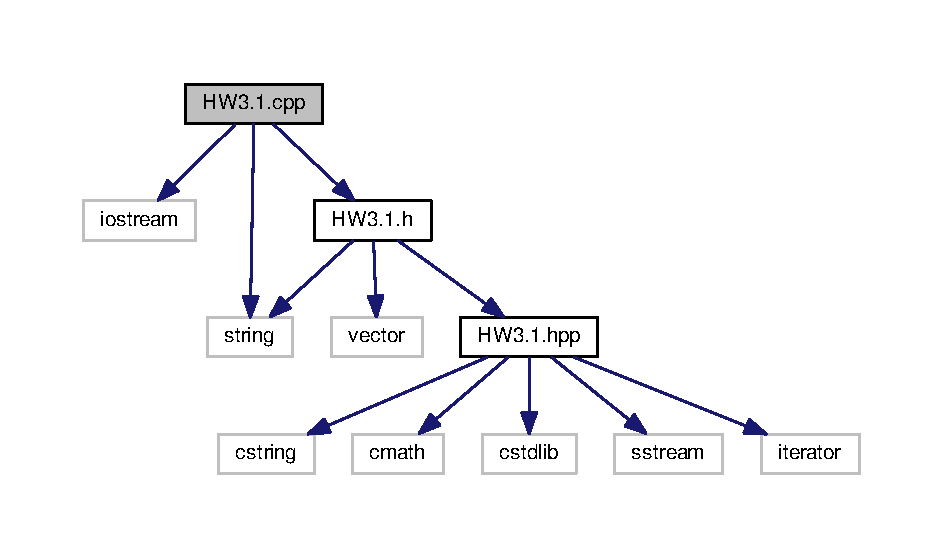
\includegraphics[width=350pt]{HW3_81_8cpp__incl}
\end{center}
\end{figure}
\subsection*{Функции}
\begin{DoxyCompactItemize}
\item 
int \hyperlink{HW3_81_8cpp_a3c04138a5bfe5d72780bb7e82a18e627}{main} (int argc, char $\ast$$\ast$argv)
\end{DoxyCompactItemize}


\subsection{Функции}
\index{H\+W3.\+1.\+cpp@{H\+W3.\+1.\+cpp}!main@{main}}
\index{main@{main}!H\+W3.\+1.\+cpp@{H\+W3.\+1.\+cpp}}
\subsubsection[{\texorpdfstring{main(int argc, char $\ast$$\ast$argv)}{main(int argc, char **argv)}}]{\setlength{\rightskip}{0pt plus 5cm}int main (
\begin{DoxyParamCaption}
\item[{int}]{argc, }
\item[{char $\ast$$\ast$}]{argv}
\end{DoxyParamCaption}
)}\hypertarget{HW3_81_8cpp_a3c04138a5bfe5d72780bb7e82a18e627}{}\label{HW3_81_8cpp_a3c04138a5bfe5d72780bb7e82a18e627}

\hypertarget{HW3_81_8h}{}\section{Файл H\+W3.1.h}
\label{HW3_81_8h}\index{H\+W3.\+1.\+h@{H\+W3.\+1.\+h}}
{\ttfamily \#include $<$string$>$}\\*
{\ttfamily \#include $<$vector$>$}\\*
{\ttfamily \#include \char`\"{}H\+W3.\+1.\+hpp\char`\"{}}\\*
Граф включаемых заголовочных файлов для H\+W3.1.h\+:\nopagebreak
\begin{figure}[H]
\begin{center}
\leavevmode
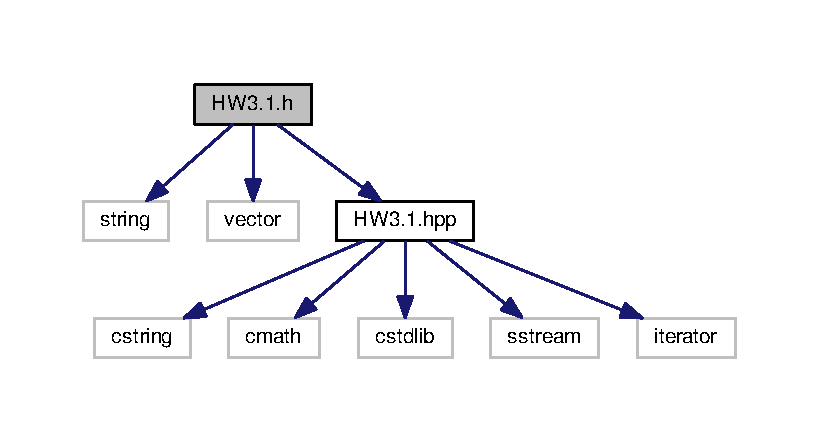
\includegraphics[width=350pt]{HW3_81_8h__incl}
\end{center}
\end{figure}
Граф файлов, в которые включается этот файл\+:\nopagebreak
\begin{figure}[H]
\begin{center}
\leavevmode
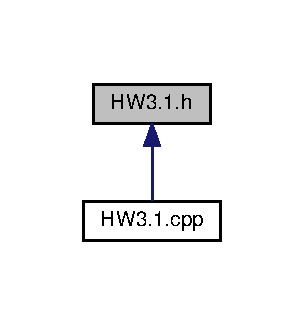
\includegraphics[width=146pt]{HW3_81_8h__dep__incl}
\end{center}
\end{figure}
\subsection*{Классы}
\begin{DoxyCompactItemize}
\item 
class \hyperlink{classWord}{Word}
\item 
class \hyperlink{classSentence}{Sentence}
\end{DoxyCompactItemize}

\hypertarget{HW3_81_8hpp}{}\section{Файл H\+W3.1.hpp}
\label{HW3_81_8hpp}\index{H\+W3.\+1.\+hpp@{H\+W3.\+1.\+hpp}}
{\ttfamily \#include $<$cstring$>$}\\*
{\ttfamily \#include $<$cmath$>$}\\*
{\ttfamily \#include $<$cstdlib$>$}\\*
{\ttfamily \#include $<$sstream$>$}\\*
{\ttfamily \#include $<$iterator$>$}\\*
Граф включаемых заголовочных файлов для H\+W3.1.hpp\+:\nopagebreak
\begin{figure}[H]
\begin{center}
\leavevmode
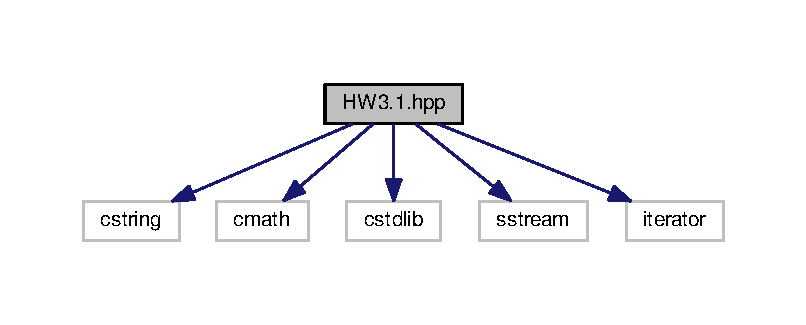
\includegraphics[width=350pt]{HW3_81_8hpp__incl}
\end{center}
\end{figure}
Граф файлов, в которые включается этот файл\+:\nopagebreak
\begin{figure}[H]
\begin{center}
\leavevmode
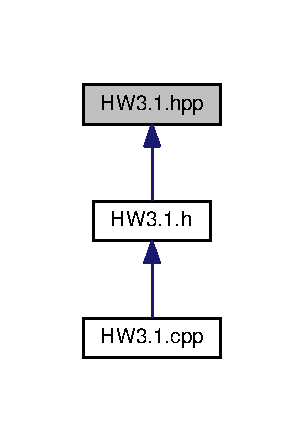
\includegraphics[width=146pt]{HW3_81_8hpp__dep__incl}
\end{center}
\end{figure}

%--- End generated contents ---

% Index
\backmatter
\newpage
\phantomsection
\clearemptydoublepage
\addcontentsline{toc}{chapter}{Алфавитный указатель}
\printindex

\end{document}
